\documentclass[10pt]{article}

\usepackage[margin=0.75in]{geometry}
\usepackage{amsmath,amsthm,amssymb}
\usepackage{xcolor}
\usepackage{cancel}
\usepackage{xcolor}
\usepackage{tikz}
\usepackage{pgfplots}
\usepackage{physics}
\usepackage{minted}
\usepackage{pythonhighlight}
\usepackage{pdfpages}
\usepackage[inline]{enumitem}

\theoremstyle{definition}
\newtheorem{problem}{Problem}
\newtheorem{soln}{Solution}

\pgfplotsset{compat=newest}

\NewDocumentCommand{\evalat}{sO{\big}mm}{%
  \IfBooleanTF{#1}
   {\mleft. #3 \mright|_{#4}}
   {#3#2|_{#4}}%
}

\title{Calculus II: Assignment 2}
\author{Jeremy Favro}
\date{\today}

\begin{document}

\maketitle

A tank has the shape of the solid of revolution obtained by revolving the curve $x = \sin(\frac{\pi y}{3})$,
for $0 \leq y \leq 3$, about the y-axis, with both axes being measured in metres. The tank is completely filled with water which is then drained from the tank at a contant rate
of 100 litres per minute. Suppose that a given instant the water in the tank is $w$ metres deep.

% PROBLEM 1
\begin{problem}
What is the volume (in litres) of the water in the tank at the given instant? Work it out both
by hand and by using SageMath.
\end{problem}
\begin{soln}
    \begin{equation}
        V(w) = \pi\int_{0}^{w} f^2(x) \,dx \text{, where f(x) is the function of the solid of revolution}
    \end{equation}
    So,
    \begin{align*}
         & = \pi\int_{0}^{w} \sin^2(\frac{\pi y}{3}) \,dy                                                                        \\
         & = \pi\int_{0}^{w} \sin^2(\frac{\pi y}{3}) \,dy \implies \text{ let } u=\frac{\pi y}{3} \text{, } dy = \frac{3du}{\pi} \\
         & = \pi\int_{0}^{w} \sin^2(u) \,\frac{3}{\pi}du                                                                         \\
         & = \cancel{\pi}\frac{3}{\cancel{\pi}}\int_{0}^{w} \sin^2(u) \,du \implies \text{ use reduction formula }               \\
         & = 3\int_{0}^{w} \left[-\frac{1}{2}\sin(u)\cos(u)+\frac{1}{2} \int_{0}^{w} \sin^0(u) \,du \right]\,du                  \\
         & = 3\int_{0}^{w} \left[-\frac{1}{2}\sin(u)\cos(u)+\frac{w}{2} \right]\,du                                              \\
         & = \eval{3\left[-\frac{1}{2}\sin(u)\cos(u)+\frac{u}{2} \right]}_0^w                                                    \\
         & = \eval{3\left[-\frac{1}{2}\sin(\frac{\pi y}{3})\cos(\frac{\pi y}{3})+\frac{\pi y}{6} \right]}_0^w                    \\
         & = -\frac{3}{2}\sin(\frac{\pi w}{3})\cos(\frac{\pi w}{3})+\frac{\pi w}{2}                                              \\
    \end{align*}

    $$\therefore V(w) = \left[-\frac{3}{2}\sin(\frac{\pi w}{3})\cos(\frac{\pi w}{3})+\frac{\pi w}{2}\right]\cdot 1000 \leftarrow \text{convert to liters} $$

    \noindent Using sage to evaluate:

    \begin{minted}[breaklines]{sage}
        clear_vars()

        y = var('y')
        w = var('w')
        
        f = sin((pi*y)/3)
        
        assume(w>0) # Has to be done to not have sage throw an error, true anyways as depth will never be negative and if it's zero volume is zero as well
        
        definite_integral(pi*f^2, y, 0, w)
    \end{minted}
\end{soln}

% PROBLEM 2
\begin{problem}
How is the depth of the water in the tank changing at the instant that the depth is 2 metres?
Work it out without implicitly or explicitly using your final answer to question 1. You may
use SageMath, or do it by hand, or mix these up.
\end{problem}
\begin{soln}
    I wasn't able to figure this out without using my answer to q1, and was unfortunately not able to make it to any of the
    office hours as they overlapped with my classes in the latter half of the week. Here's the couple pages of work (ramblings) I did in trying to solve it in case that counts:
    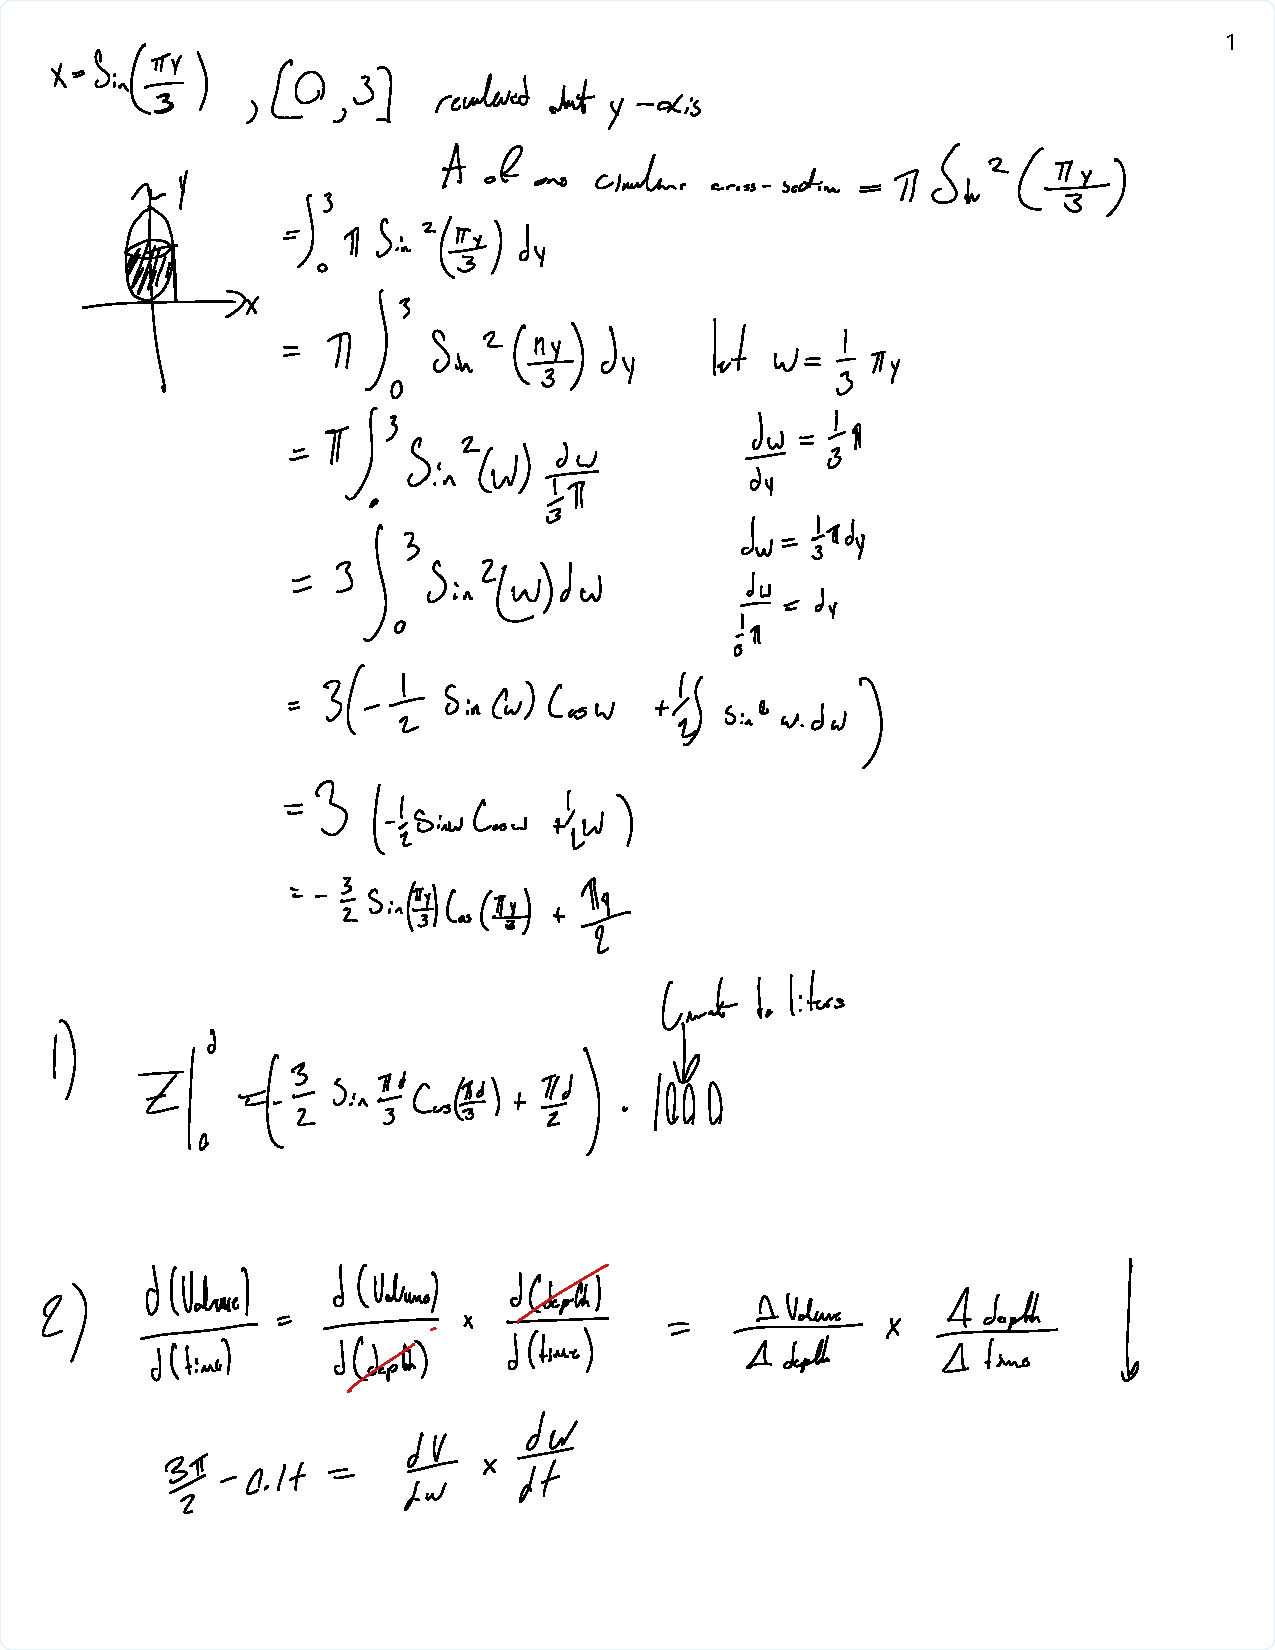
\includepdf[pages=-]{MATH_1120H_A2.pdf}

\end{soln}
\end{document}